\documentclass{article}
\usepackage[T1]{fontenc}
\usepackage{lmodern}
\usepackage{graphicx}
\usepackage{amsmath,amssymb}
\usepackage[a4paper,margin=2cm]{geometry}
\usepackage[absolute,overlay]{textpos}
\setlength{\TPHorizModule}{1mm}
\setlength{\TPVertModule}{1mm}
\usepackage[indonesian]{babel}
\usepackage{hyperref}
\setlength{\emergencystretch}{2em}
% unit: Halaman 19

\begin{document}

% === Halaman 19 (llm) ===

\vspace{151.47mm}

\vspace{50mm}
\begin{center}
Transformasi $SubBytes$
\end{center}

% deskripsi: Diagram proses transformasi SubBytes pada AES yang menunjukkan pemetaan dari sebuah matriks 'state' (elemen a_ij) melalui sebuah S-box menjadi matriks 'state'' (elemen b_ij).
% bbox normalisasi: [0.1400, 0.1500, 0.8400, 0.6600]
\begin{textblock*}{147.00mm}(29.40mm,44.55mm)
\noindent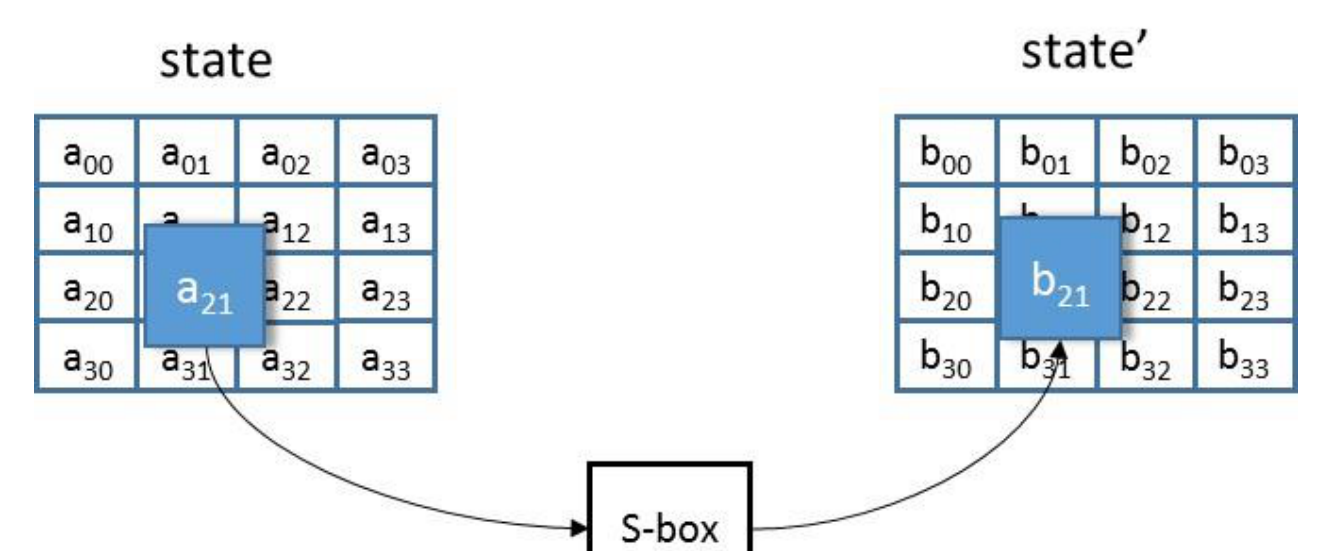
\includegraphics[width=147.00mm,height=151.47mm]{../../images/llm/page_019_img_01.png}%
\end{textblock*}

\end{document}
